%% start of file `template.tex'.
%% Copyright 2006-2015 Xavier Danaux (xdanaux@gmail.com), 2020-2022 moderncv maintainers (github.com/moderncv).
%
% This work may be distributed and/or modified under the
% conditions of the LaTeX Project Public License version 1.3c,
% available at http://www.latex-project.org/lppl/.


\documentclass[10pt,a4paper,sans]{moderncv}        % possible options include font size ('10pt', '11pt' and '12pt'), paper size ('a4paper', 'letterpaper', 'a5paper', 'legalpaper', 'executivepaper' and 'landscape') and font family ('sans' and 'roman')

% moderncv themes
\moderncvstyle{classic}                             % style options are 'casual' (default), 'classic', 'banking', 'oldstyle' and 'fancy'
\moderncvcolor{blue}                               % color options 'black', 'blue' (default), 'burgundy', 'green', 'grey', 'orange', 'purple' and 'red'
%\renewcommand{\familydefault}{\sfdefault}         % to set the default font; use '\sfdefault' for the default sans serif font, '\rmdefault' for the default roman one, or any tex font name
\nopagenumbers{}                                  % uncomment to suppress automatic page numbering for CVs longer than one page

% adjust the page margins
\usepackage[scale=0.75]{geometry}
%\setlength{\footskip}{136.00005pt}                 % depending on the amount of information in the footer, you need to change this value. comment this line out and set it to the size given in the warning
%\setlength{\hintscolumnwidth}{3cm}                % if you want to change the width of the column with the dates
%\setlength{\makecvheadnamewidth}{10cm}            % for the 'classic' style, if you want to force the width allocated to your name and avoid line breaks. be careful though, the length is normally calculated to avoid any overlap with your personal info; use this at your own typographical risks...

% font loading
% for luatex and xetex, do not use inputenc and fontenc
% see https://tex.stackexchange.com/a/496643
\ifxetexorluatex
  \usepackage{fontspec}
  \usepackage{unicode-math}
  \defaultfontfeatures{Ligatures=TeX}
  \setmainfont{Latin Modern Roman}
  \setsansfont{Latin Modern Sans}
  \setmonofont{Latin Modern Mono}
  \setmathfont{Latin Modern Math} 
\else
  \usepackage[T1]{fontenc}
  \usepackage{lmodern}
\fi

% document language
\usepackage[german]{babel}  % FIXME: using spanish breaks moderncv
% only include pages in range in pdf
%\usepackage[1]{pagesel} % Anschreiben
%\usepackage[2]{pagesel} % Lebenslauf
%\usepackage[3-5]{pagesel} % Arbeitszeugnis
%\usepackage[6-7]{pagesel} % Notenübersicht

\usepackage{pdfpages}
% personal data
\name{Lukas-Angelo}{Meier}
%\title{Résumé title}                               % optional, remove / comment the line if not wanted
\born{4. Mai 1993}                                 % optional, remove / comment the line if not wanted
\address{Bahnhofstraße 32}{33102 Paderborn}{}       % optional, remove / comment the line if not wanted; the "postcode city" and "country" arguments can be omitted or provided empty
\phone[mobile]{+49~(162)~829~4802}                   % optional, remove / comment the line if not wanted; the optional "type" of the phone can be "mobile" (default), "fixed" or "fax"
%\phone[fixed]{+2~(345)~678~901}
%\phone[fax]{+3~(456)~789~012}
\email{lukas-angelo.meier@proton.me}                               % optional, remove / comment the line if not wanted
%\homepage{www.johndoe.com}                         % optional, remove / comment the line if not wanted

% Social icons
%\social[linkedin]{john.doe}                        % optional, remove / comment the line if not wanted
%\social[xing]{john\_doe}                           % optional, remove / comment the line if not wanted
%\social[twitter]{ji\_doe}                             % optional, remove / comment the line if not wanted
%\social[github]{jdoe}                              % optional, remove / comment the line if not wanted
%\social[gitlab]{jdoe}                              % optional, remove / comment the line if not wanted
% \social[stackoverflow]{0000000/johndoe}            % optional, remove / comment the line if not wanted
% \social[bitbucket]{jdoe}                           % optional, remove / comment the line if not wanted
% \social[skype]{jdoe}                               % optional, remove / comment the line if not wanted
% \social[orcid]{0000-0000-000-000}                  % optional, remove / comment the line if not wanted
% \social[researchgate]{jdoe}                        % optional, remove / comment the line if not wanted
% \social[researcherid]{jdoe}                        % optional, remove / comment the line if not wanted
% \social[telegram]{jdoe}                            % optional, remove / comment the line if not wanted
% \social[whatsapp]{12345678901}                     % optional, remove / comment the line if not wanted
% \social[signal]{12345678901}                       % optional, remove / comment the line if not wanted
% \social[matrix]{@johndoe:matrix.org}               % optional, remove / comment the line if not wanted
% \social[googlescholar]{googlescholarid}            % optional, remove / comment the line if not wanted


%\extrainfo{additional information}                 % optional, remove / comment the line if not wanted
%\photo[64pt][0.4pt]{picture}                       % optional, remove / comment the line if not wanted; '64pt' is the height the picture must be resized to, 0.4pt is the thickness of the frame around it (put it to 0pt for no frame) and 'picture' is the name of the picture file
%\quote{Some quote}                                 % optional, remove / comment the line if not wanted

% bibliography adjustments (only useful if you make citations in your resume, or print a list of publications using BibTeX)
%   to show numerical labels in the bibliography (default is to show no labels)
%\makeatletter\renewcommand*{\bibliographyitemlabel}{\@biblabel{\arabic{enumiv}}}\makeatother
\renewcommand*{\bibliographyitemlabel}{[\arabic{enumiv}]}
%   to redefine the bibliography heading string ("Publications")
%\renewcommand{\refname}{Articles}

% bibliography with mutiple entries
%\usepackage{multibib}
%\newcites{book,misc}{{Books},{Others}}
%----------------------------------------------------------------------------------
%            content
%----------------------------------------------------------------------------------
\begin{document}
%\begin{CJK*}{UTF8}{gbsn}                          % to typeset your resume in Chinese using CJK
%-----       letter       ---------------------------------------------------------
% recipient data
\recipient{Bewerbung als Studentische Hilfskraft in der Hausnotruf-Verwaltung}{Malteser Hilfsdienst e.V.\\
Erna-Scheffler-Str. 2\\
51103 Köln }
\date{\today}
\opening{Sehr geehrte Frau Haselhorst,}
\closing{Mit freundlichem Gruß,}
\enclosure[Anhang]{Lebenslauf, Arbeitszeugnis, Notenübersicht}          % use an optional argument to use a string other than "Enclosure", or redefine \enclname
\makelettertitle

hiermit bewerbe ich mich als studentische Hilfskraft in der Hausnotruf-Verwaltung am Standort Paderborn. 
Aktuell studiere ich Informatik und bringe neben einer strukturierten und zuverlässigen Arbeitsweise 
auch gute organisatorische Fähigkeiten mit.

Mich motiviert vor allem, mit meiner Tätigkeit einen konkreten Beitrag zur Unterstützung 
hilfsbedürftiger Menschen zu leisten und gleichzeitig Einblicke in die Praxis sozialer Dienstleistungen 
zu gewinnen. Der Umgang mit Menschen sowie administrative Aufgaben liegen mir gleichermaßen.

Gerne unterstütze ich Ihr Team engagiert und verantwortungsbewusst und freue mich auf
 die Gelegenheit, mich persönlich vorzustellen.

\makeletterclosing

\clearpage

%-----       resume       ---------------------------------------------------------
\makecvtitle

%\section{Master thesis}
%\cvitem{title}{\emph{Title}}
%\cvitem{supervisors}{Supervisors}
%\cvitem{description}{Short thesis abstract}

\section{Berufserfahrung}
%\subsection{Vocational}
\cventry{11.2025--02.2026}{SHK}{Flaschenpost}{Bielefeld}{}{
  \begin{itemize}
\item Zuverlässige Auslieferung von Bestellungen unter Zeitdruck
\item Direkter Kundenkontakt und serviceorientiertes Auftreten
\item Eigenständige Organisation von Touren und Arbeitsabläufen
\end{itemize}
}
\cventry{2019--2025}{Werkstudent – IT-Sicherheit und sichere IoT-Systeme}{Fraunhofer IEM}{Paderborn}{}{
\begin{itemize}
%\item Statische Codeanalyse großer C/C++ Codebasen
%  \begin{itemize}
%    \item Analyse der Open-Source-OPC-UA Implementierung open62541 mittels statischer Analysewerkzeuge.
%    \item Manuelle Evaluation der Analyseergebnisse zur Identifikation sicherheitsrelevanter Schwachstellen.
%  \end{itemize}
%\item Netzwerk- und Protokollanalyse
%  \begin{itemize}
%    \item Entwicklung eines Python-basierten Tools zur Analyse von OPC-UA Netzwerkverkehr.
%    \item Analyse und Manipulation von Netzwerkpaketen zur Untersuchung sicherheitskritischer Kommunikationsszenarien.
%  \end{itemize}
%\item Forschungsprototyp zur Bedrohungsanalyse
%  \begin{itemize}
%    \item Mitarbeit an der Entwicklung eines Java-basierten Forschungsprototypen zur automatischen Identifikation von Bedrohungen.
%    \item Weiterentwicklung eines Metamodells zur Beschreibung komplexer Systemarchitekturen und Kommunikationsstrukturen.
%  \end{itemize}
%\item Demonstrator zur Log4j-Sicherheitslücke
%  \begin{itemize}
%    \item Entwicklung eines Demonstrators zur Veranschaulichung der Log4j-Schwachstelle.
%    \item Implementierung eines Web-Dashboards zur Visualisierung von Angriffsszenarien.
%  \end{itemize}
\item Analyse komplexer Softwarekomponenten sowie strukturierte Auswertung von Ergebnissen
\item Sorgfältige und eigenständige Bearbeitung von Aufgaben in Forschungsprojekten
\item Dokumentation und Aufbereitung technischer Sachverhalte für unterschiedliche Zielgruppen
\item Entwicklung von Tools zur Unterstützung von Analyse- und Auswertungsprozessen
\item Enge Zusammenarbeit im Team sowie Abstimmung mit verschiedenen Projektbeteiligten
\end{itemize}
}
%\subsection{Miscellaneous}
\cventry{2016--2019}{SHK}{Vetter+Engels}{Paderborn}{}{Kommissionierer}


\section{Studium}
\cventry{2013--heute}{B.Sc. Informatik}{Universität Paderborn}{Paderborn}{}{}  % arguments 3 to 6 can be left empty
\cventry{2012--2013}{Bachelor Elektrotechnik}{Universität Paderborn}{Paderborn}{}{}
\cventry{2010--2012}{Abitur}{CJD Oberurff}{Oberurff}{}{}
\cventry{2003--2010}{Gymnasium}{Gustav Stresemann Gymnasium}{Bad Wildungen}{}{}


\section{Sprachkenntnisse}
\cvitemwithcomment{Deutsch}{Muttersprache}{}
\cvitemwithcomment{Englisch}{C1}{}
%\cvitemwithcomment{Language 4}{Skill level}{Comment}

%\section{Computer skills}
%\cvdoubleitem{category 1}{XXX, YYY, ZZZ}{category 4}{XXX, YYY, ZZZ}
%\cvdoubleitem{category 2}{XXX, YYY, ZZZ}{category 5}{XXX, YYY, ZZZ}
%\cvdoubleitem{category 3}{XXX, YYY, ZZZ}{category 6}{XXX, YYY, ZZZ}

\section{Skill Matrix}
%\cvitem{Skill matrix}{Alternatively, provide a skill matrix to show off your skills}
%% Skill matrix as an alternative to rate one's skills, computer or other. 

%% Adjusts width of skill matrix columns. 
%% Usage \setcvskillcolumns[<width>][<factor>][<exp_width>]
%% <width>, <exp_width> should be lengths smaller than \textwidth, <factor> needs to be between 0 and 1.
%% Examples:
%\setcvskillcolumns[5em][][]%    adjust first column. Same as \setcvskillcolumns[5em]
\setcvskillcolumns[][0.6][]%   adjust third (skill) column. Same as \setcvskillcolumns[][0.45]
% \setcvskillcolumns[][][\widthof{``Year''}]%     adjust fourth (years) column.
% \setcvskillcolumns[][0.45][\widthof{``Year''}]%
% \setcvskillcolumns[\widthof{``Languag''}][0.48][]
% \setcvskillcolumns[\widthof{``Languag''}]%

%% Adjusts width of legend columns. Usage \setcvskilllegendcolumns[<width>][<factor>]
%% <factor> needs to be between 0 and 1. <width> should be a length smaller than \textwidth
%% Examples:
% \setcvskilllegendcolumns[][0.45]
% \setcvskilllegendcolumns[\widthof{``Legend''}][0.45]
% \setcvskilllegendcolumns[0ex][0.46]% this is usefull for the banking style

%% Add a legend if you are using \cvskill{<1-5>} command or \cvskillentry
%% Usage \cvskilllegend[*][<post_padding>][<first_level>][<second_level>][<third_level>][<fourth_level>][<fifth_level>]{<name>}
% \cvskilllegend % insert default legend without lines
%\cvskilllegend*[1em]{}% adjust post spacing
% \cvskilllegend*{Legend}%  Alternatively add a description string
%% adjust the legend entries for other languages, here German
% \cvskilllegend[0.2em][Grundkenntnisse][Grundkenntnisse und eigene Erfahrung in Projekten][Umfangreiche Erfahrung in Projekten][Vertiefte Expertenkenntnisse][Experte\,/\,Spezialist]{Legende}

%% Alternative legend style with the first three skill levels in one column
%% Usage \cvskillplainlegend[*][<post_padding>][<first_level>][<second_level>][<third_level>][<fourth_level>][<fifth_level>]{<name>}
% \setcvskilllegendcolumns[][0.6]%  works for classic, casual, banking
% \setcvskilllegendcolumns[][0.55]%  works better for oldstyle and fancy
% \cvskillplainlegend{}
% \cvskillplainlegend[0.2em][Grundkenntnisse][Grundkenntnisse und eigene Erfahrung in Projekten][Umfangreiche Erfahrung in Projekten][Vertiefte Expertenkenntnisse][Experte/Guru]{Legende}

%% Add a head of the skill matrix table with descriptions.
%% Usage \cvskillhead[<post_padding>][<Level>][<Skill>][<Years>][<Comment>]%
%\cvskillhead[-0.1em]%   this inserts the standard legend in english and adjust padding
%% Adjust head of the skill matrix for other languages
% \cvskillhead[0.25em][Level][F\"ahigkeit][Jahre][Bemerkung]

%% \cvskillentry[*][<post_padding>]{<skill_cathegory>}{<0-5>}{<skill_name>}{<years_of_experience>}{<comment>}% 
%% Example usages:
\cvskillentry*{Office:}{4}{MS Office}{}{}
\cvskillentry*{Sprachen:}{4}{Java, Python}{}{}
\cvskillentry{}{3}{C/C++, Bash}{}{}
\cvskillentry{}{2}{SQL, HTML, CSS, JavaScript, PHP}{}{}
\cvskillentry*{OS:}{4}{Linux}{}{}% notice the use of the starred command and the optional 
\cvskillentry*{Sonstiges:}{3}{Git, \LaTeX}{}{}
%% \cvskill{<0-5>} command
% \cvitem{\textbackslash{cvskill}:}{Skills can be visually expressed by the \textbackslash{cvskill} command, e.g. \cvskill{2}}

%\section{Interessen}
%\cvitem{Hacking}{Seit einigen Jahren Mitglied bei /upb/hack und an mehreren CTFs, remote sowie onsite, teilgenommen.}
%\cvitem{hobby 2}{Description}
%\cvitem{hobby 3}{Description}

%\section{Extra 1}
%\cvlistitem{Item 1}
%\cvlistitem{Item 2}
%\cvlistitem{Item 3. This item is particularly long and therefore normally spans over several lines. Did you notice the indentation when the line wraps?}

%\section{Extra 2}
%\cvlistdoubleitem{Item 1}{Item 4}
%\cvlistdoubleitem{Item 2}{Item 5\cite{book2}}
%\cvlistdoubleitem{Item 3}{Item 6. Like item 3 in the single column list before, this item is particularly long to wrap over several lines.}

%\section{References}
%\begin{cvcolumns}
%  \cvcolumn{Category 1}{\begin{itemize}\item Person 1\item Person 2\item Person 3\end{itemize}}
%  \cvcolumn{Category 2}{Amongst others:\begin{itemize}\item Person 1, and\item Person 2\end{itemize}(more upon request)}
%  \cvcolumn[0.5]{All the rest \& some more}{\textit{That} person, and \textbf{those} also (all available upon request).}
%\end{cvcolumns}

% Publications from a BibTeX file without multibib
%  for numerical labels: \renewcommand{\bibliographyitemlabel}{\@biblabel{\arabic{enumiv}}}% CONSIDER MERGING WITH PREAMBLE PART
%  to redefine the heading string ("Publications"): \renewcommand{\refname}{Articles}
%\nocite{*}
%\bibliographystyle{plain}
%\bibliography{publications}                        % 'publications' is the name of a BibTeX file

% Publications from a BibTeX file using the multibib package
%\section{Publications}
%\nocitebook{book1,book2}
%\bibliographystylebook{plain}
%\bibliographybook{publications}                   % 'publications' is the name of a BibTeX file
%\nocitemisc{misc1,misc2,misc3}
%\bibliographystylemisc{plain}
%\bibliographymisc{publications}                   % 'publications' is the name of a BibTeX file

%\clearpage\end{CJK*}                              % if you are typesetting your resume in Chinese using CJK; the \clearpage is required for fancyhdr to work correctly with CJK, though it kills the page numbering by making \lastpage undefined

% Weitere PDF dokumente einfügen

\includepdf[pages=-]{Arbeitszeugnis_IEM.pdf}
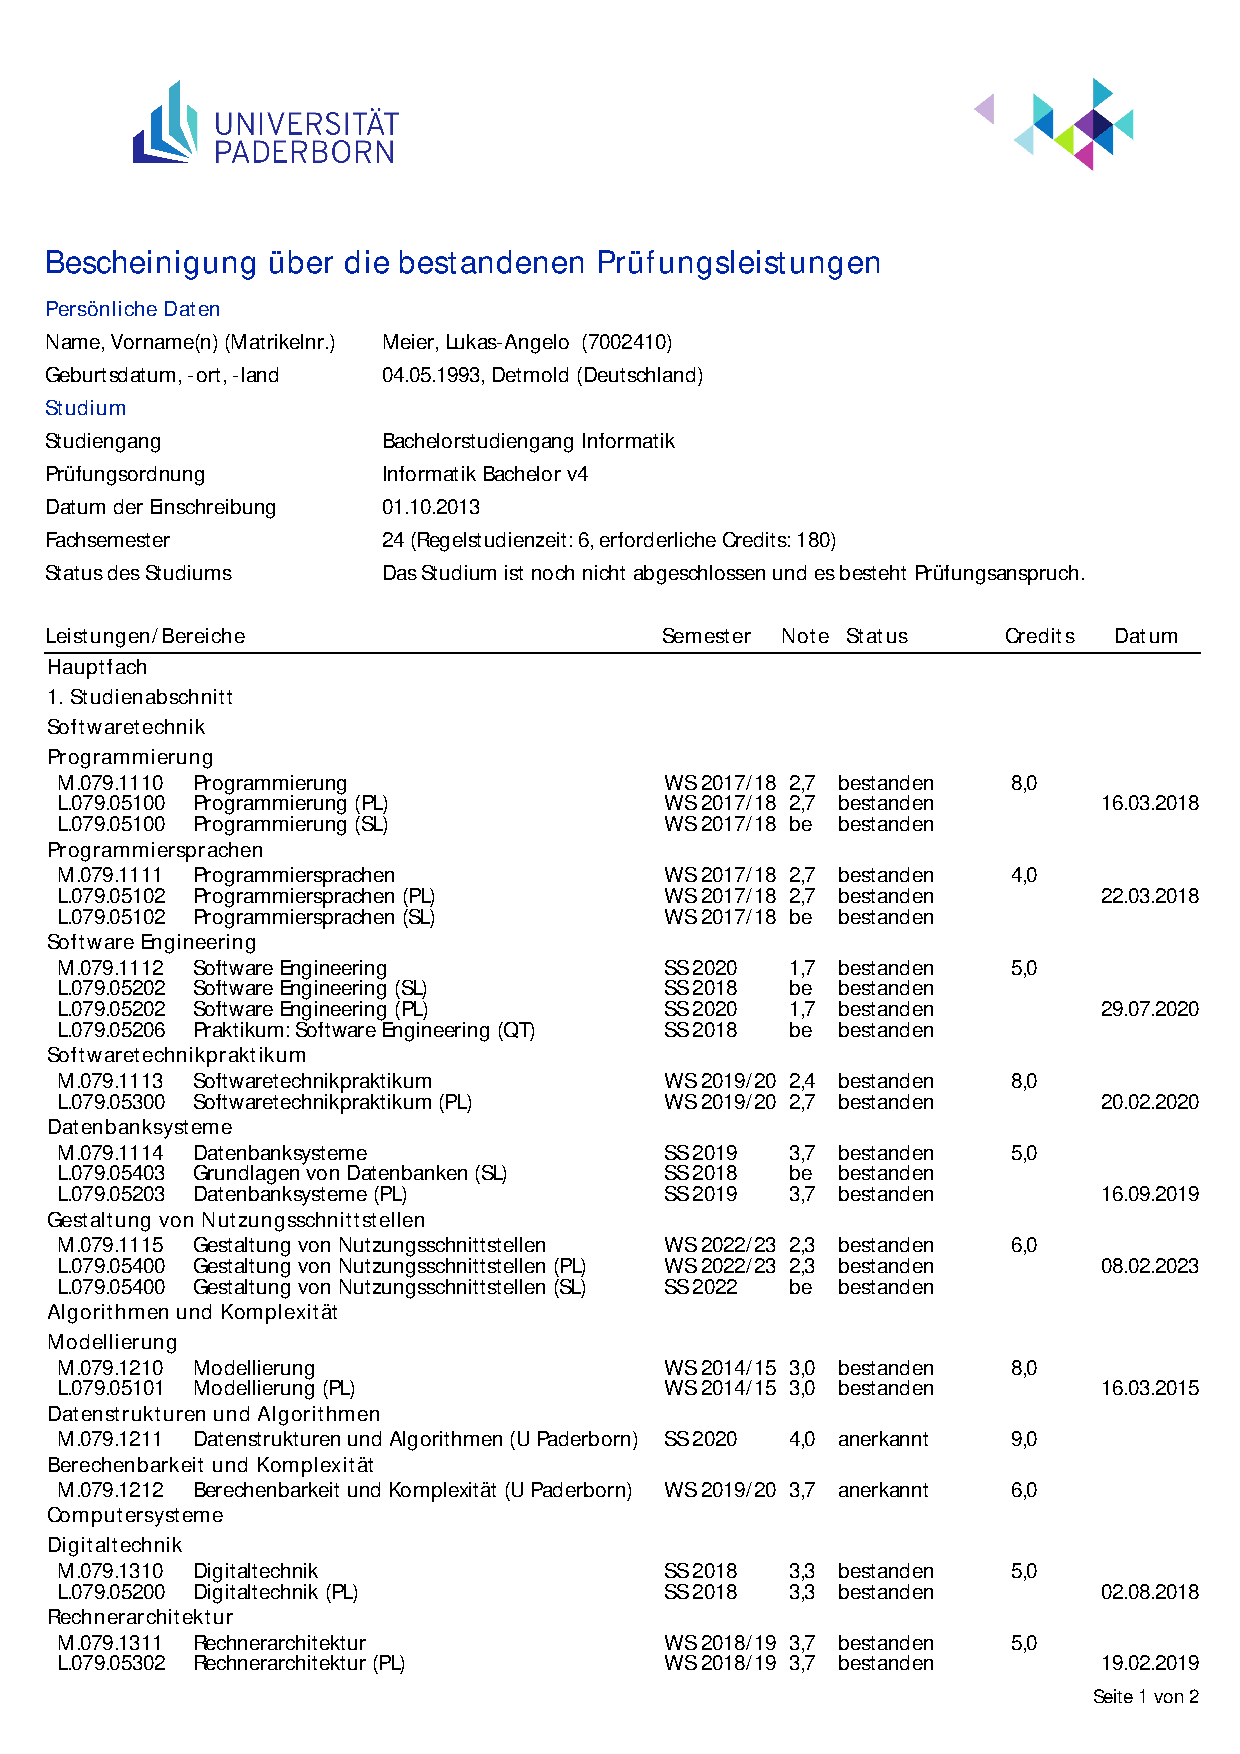
\includepdf[pages=-]{Leistungsübersicht.pdf}

\end{document}


%% end of file `template.tex'.

